\section{Conceptos previos}
En este apartado se describe la arquitectura de VMware Cloud Foundation y como estructura sus componentes\footnote{Se describen solo aquellos componentes que se utilizarán en el despliegue de Cloud Foundation.} internamente.

%%%%%%%%%%%%%%%%%%%%%%%%%%%%%%
\iffalse
En este apartado se explican aquellos conceptos de VMware Cloud Foundation necesarios para entender su funcionamiento, configuración y requisitos de la infraestructura previos al despliegue del servicio.
\fi
%%%%%%%%%%%%%%%%%%%%%%%%%%%%%%%%


%% Workload Ddomains %&%&%%%%
%%%%%%%%%%%%%%%%%%%%%%%%%%%%
\subsection{Workload Domain}
Un \textit{workload domain} (WD) representa un bloque de recursos dentro del SDDC, que son componentes de la infraestructura física, de la infraestructura virtual, y de seguridad. Los componentes virtuales controlan el acceso y la reserva de los recursos físicos, mientras que la capa de seguridad permite establecer organizar la entrada al WD. Cada WD contiene sus propias instancias de VMware ESXi, VMware vCenter Server, VMware NSX-T y VMware vSAN, pudiendo así gestionar los recursos de cada WD de forma independiente.
% Un \textit{workload domain} consiste en una instancia lógica de un SDDC que abarca todos o parte de los recursos de uno o más clusters, cuya función es aislar el flujo de trabajo de un usuario, aplicación o un determinado tipo de tareas. Cada \textit{workload domain} se extiende sobre varios hosts con el hipervisor ESXi, y contiene sus propias instancias de VMware vCenter Server, VMware vSAN y VMware NSX-T. Así, esta arquitectura permite establecer políticas de control específicas para un \textit{workload domain} y otras comunes para todos o varios \textit{workload domains} y específicas para cada uno de ellos a la vez que se simplifica la complejidad de la infraestructura. Existen \underline{tres tipos} de \textit{workload domains} que permiten aislar las tareas de gestión de la infraestructura del resto de flujos de trabajo. 

%% MANAGEMENT DOMAIN
\subsubsection{Management Domain}
\label{subsubsec:domainManagement}
% Este \textit{workload domain} se crea y configura automáticamente durante el proceso de despliegue de una instancia de VMware Cloud Foundation.
El \textit{management domain} es el primer WD que se crea dentro del SDDC, y su función es la gestión de todos los componentes de VMware Cloud Foundation, tanto del propio \textit{management domain} como del resto de \textit{workload domains} existentes. Aparte de las instancias descritas, este WD incluye una instancia de SDDC Manager.

% Incluye las siguientes instancias: SDDC Manager, vCenter Server, una instancia de NSX Manager, tres instancias de NSX Controller, dos instancias de Platform Services Controller y tres instancias de vRealize Log Insight \cite{sddcComponents} [Fig. \ref{fig:componentsMNGDomain}].\\
% Cuando se \underline{despliega \textit{management domain} se crean y configuran} de forma automatizada por SDDC Manager las siguientes máquinas virtuales (VM) de cada componente de Cloud Foundation\footnote{Las características de cada máquina virtual se refieren a los requisitos mínimos}:
% \begin{itemize}
%     \item Una VM de \textbf{SDDC Manager}: 4 vCPU, 16 GB de memoria, 800 GB de almacenamiento.
%     \item Una VM de \textbf{vCenter Server}: 4 vCPU, 16 GB de memoria, 290 GB de almacenamiento.
%     \item Dos instancias de \textbf{Platform Services Controller} (cada una): 2 vCPU, 4 GB de memoria, 60 GB de almacenamiento.
%     \item Una VM de \textbf{NSX Manager}: 4 vCPU, 16 GB de memoria, 60 GB de almacenamiento.
%     \item Tres VM de \textbf{NSX Controller} (cada una): 4 vCPU, 4 GB de memoria, 28 GB de almacenamiento.
%     \item Tres VM de \textbf{vRealize Log Insight}: 4 vCPU, 8 GB de memoria, 250 GB de almacenamiento.
% \end{itemize}

Para desplegar el \textit{management domain} se requieren las siguientes \underline{capacidades mínimas} en la infraestructura \cite{WDminRequierements}:
\begin{itemize}
    \item \textbf{Hosts}: 4
    \item \textbf{CPU} por host: Dual-socket con 8 cores por socket, en sistemas All-Flash.
    \item \textbf{Memoria} total: 192 GB
    \item \textbf{Almacenamiento} por host: 16 GB para el dispositivo de arranque, un NVMe o SSD para la capa de caché, dos SSD o HDD para la capa de capacidad\footnote{En total se requieren 800 GB para este \textit{workload domain}.}.
    \item \textbf{NICs} por host: Dos NICs de al menos 10 GbE y, opcionalmente un NIC 1GbE BMC.
\end{itemize}

\begin{figure}[h!]
  \centering
  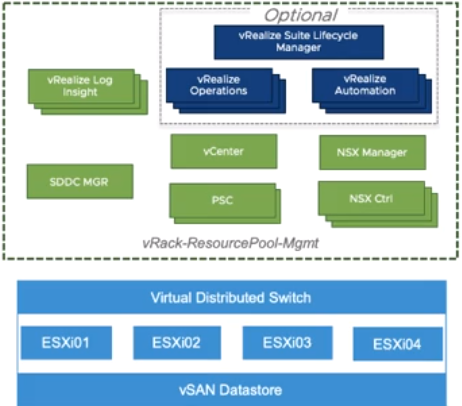
\includegraphics[width=0.5\textwidth]{imaxes/conceptosPrevios/componentsMANAGEDomain.png}
  \caption{Componentes de \textit{management domain}}
  \label{fig:componentsMNGDomain}
\end{figure}
\FloatBarrier 


%% VIRTUAL INF. DOMAIN
\begin{subsubsection}{Virtual Infrastructure Domain (VI) y Virtual Desktop Infrastructure Domain (VDI)}
\label{subsubsec:domainVI}
Este tipo de \textit{workload domain} se crea manualmente y bajo demanda desde \textit{management domain} para dar servicio a las necesidades de cada usuario o para crear diferentes entornos con finalidades distintas. Su configuración de hardware y lógica se especifican durante su proceso de creación, permitiendo indicar la cantidad de hosts, cantidad de almacenamiento, configuración de la red y políticas de rendimiento y disponibilidad, todo para satisfacer las necesidades del tipo de tareas para las que se crea. El acceso a un \textit{VI domain} se realiza a través de vSphere Client donde el administrador puede gestionar todos los recursos asociados con ese \textit{workload domain}. Cada \textit{virtual infrastructure domain} cuenta con sus propios vCenter Server y un NSX Manager dedicados, que se ejecutan desde el \textit{management domain} de la infraestructura, y \textit{datastore} vSAN dedicado. La diferencia entre un \textit{virtual infrastructure domain} y \textit{virtual desktop infrastructure domain} es que el segundo incorpora el producto VMware Horizon View que, resumiendo, permite desplegar escritorios virtuales. Con cada nuevo \textit{virtual infrastructure domain} se crea un nuevo cluster vSphere en la infraestructura que agrupa todos los recursos que tiene asignados.\\
Cuando se \underline{despliega un \textit{virtual infrastructure domain} se crean y configuran} de forma automatizada por el componente SDDC Manager las siguientes máquinas virtuales (VM) de cada componente de VMware Cloud Foundation\footnote{Las características de cada máquina virtual se refieren a los requisitos mínimos} \cite{sddcComponents} [Fig. \ref{fig:compoVIdomain}]:
\begin{itemize}
    \item Una VM de \textbf{vCenter Server} en Management Domain: 8 vCPU, 24 GB de memoria, 500 GB de almacenamiento.
    \item Una VM de \textbf{NSX Manager} en Management Domain: 4 vCPU, 16 GB de memoria, 60 GB de almacenamiento.
    \item Tres VM de \textbf{NSX Controller} en el VI Domain creado (cada una):  4 vCPU, 4 GB de memoria, 28 GB de almacenamiento.
\end{itemize}

Por cada \textit{virtual infraestructure domain} que se despliega en la infraestructura, se requieren las siguientes capacidades mínimas\cite{WDminRequierements}:
\begin{itemize}
    \item \textbf{Hosts}: 3
    \item \textbf{CPU}, \textbf{Memoria} y \textbf{Almacenamiento}: depende de los requisitos de las tareas que se vayan a desarrollar en este \textit{workload domain}.
    \item \textbf{NICs} por servidor: Dos NICs de al menos 10 GbE y, opcionalmente un NIC 1 GbE BMC.
\end{itemize}


\end{subsubsection}

\begin{figure}[h!]
  \centering
  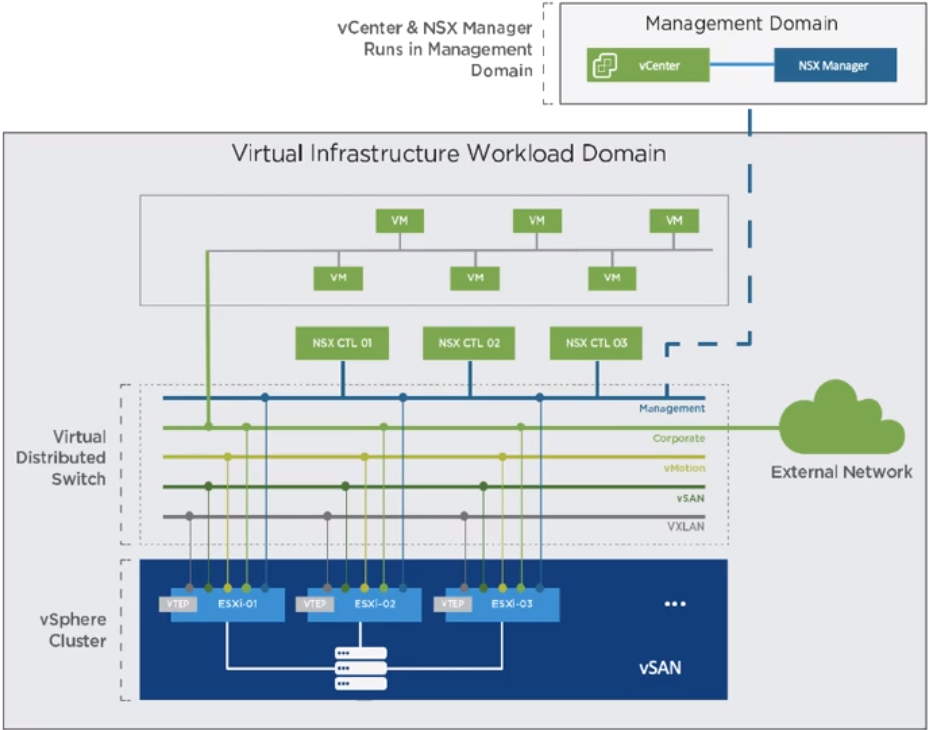
\includegraphics[width=0.5\textwidth]{imaxes/conceptosPrevios/networkArcVIDomain.png}
  \caption{Componentes de \textit{virtual infrastructure domain}.}
  \label{fig:compoVIdomain}
\end{figure}
\FloatBarrier

%&%%%%%%%%%%%%%%%%%%%%%%%%%%%%%%%%%%%%%%%%%%%%%%%%%%%%%%%%
%% ARQUITECTURA



\subsection{Arquitectura}
La arquitectura de VMware Cloud Foundation tiene dos posibles modelos de despliegue dependiendo del número de hosts sobre los que se despliega VMware Cloud Foundation.

%% ESTANDAR
\subsubsection{Modelo estándar}
Este modelo está pensado para desplegar VMware Cloud Foundation en entornos de tamaño medio/grande con un mínimo de siete hosts. Está formado por un \textit{management domain} que se despliega en cuatro de los hosts y contiene todos los componentes de gestión de toda la infraestructura, desde este \textit{workload domain} se administra la infraestructura del SDDC y cada \textit{virtual infrastructure domain} existente. Además, este modelo contiene al menos un \textit{virtual infrastructure domain}, creado bajo demanda y con capacidades establecidas según su finalidad que posteriormente se pueden pueden modificar, se despliega sobre al menos tres hosts. Cada \textit{virtual infrastructure domain} requiere tres hosts adicionales, es decir, un host solo puede pertenecer a un único \textit{workload domain}. El máximo número de \textit{virtual infrastructure domains} que se pueden desplegar en una instacia de VMware Cloud Foundation es 14.

\begin{figure}[h!]
  \centering
  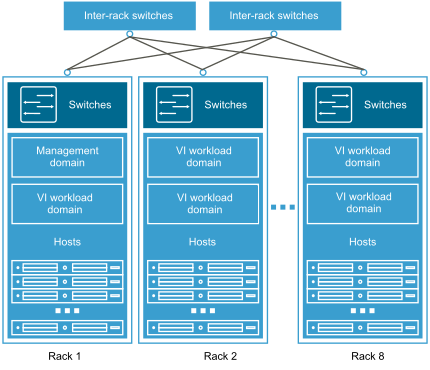
\includegraphics[width=0.6\textwidth]{imaxes/conceptosPrevios/arquitect_standarCF.png}
  \caption{Esquema del modelo de arquitectura estándar.}
  \label{fig:modelostandard}
\end{figure}

\begin{figure}[h!]
  \centering
  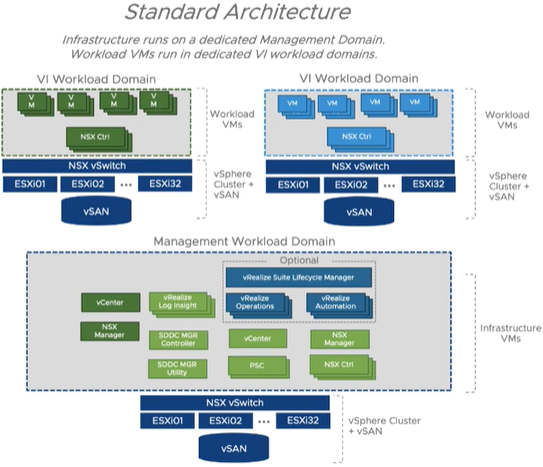
\includegraphics[width=0.6\textwidth]{imaxes/conceptosPrevios/standardArch.png}
  \caption{Estructura de los componentes en una arquitectura estándar.}
  \label{fig:standardarch}
\end{figure}
\FloatBarrier
%%%%%%%%%%%%%%%%%%%%%
%%  CONSOLIDADO
\subsubsection{Modelo consolidado}
Este modelo está pensado para desplegar VMware Cloud Foundation en entornos de tamaño pequeño, normalmente cuando hay menos de siete hosts, aunque se puede también se puede utilizar sobre entornos más grandes de hasta 64 hosts. En este modelo los flujos de trabajo que corresponden al \textit{virtual infrastructure domain} y al \textit{management domain} en el despliegue estándar, están colocados dentro de un mismo \textit{workload domain} en un único cluster pero aislados gracias a que cada uno se coloca dentro de un \textit{resource pool}, es decir, solo existe un cluster con varios \textit{resource pool}. Un \textit{resource pool} es una carcaterística de VMware vSphere que permite abstraer un conjunto de recursos de un cluster estableciendo unos límites de capacidad que puede usar \cite{resourcePool}. Este modelo se puede convertir en un modelo estándar creando un \textit{virtual infrastructure domain}.[Fig. \ref{fig:modeloconsolidated}].

\begin{figure}[h!]
  \centering
  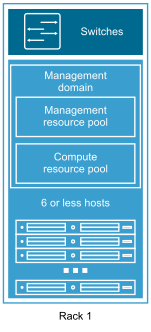
\includegraphics[width=0.25\textwidth]{imaxes/conceptosPrevios/modelConsolidated.png}
  \caption{Esquema del modelo de arquitectura consolidado.}
  \label{fig:modeloconsolidated}
\end{figure}

\begin{figure}[h!]
  \centering
  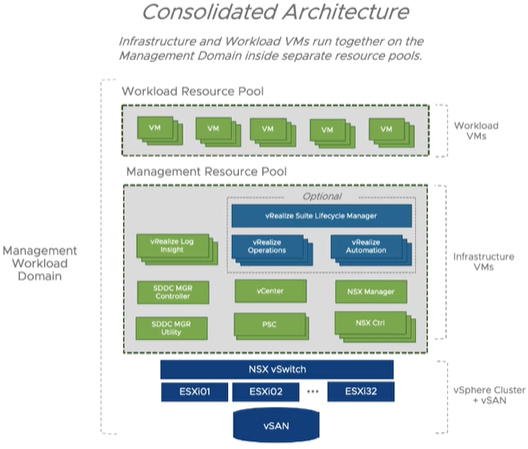
\includegraphics[width=0.85\textwidth]{imaxes/conceptosPrevios/consolidatedArch.png}
  \caption{Estructura de los componentes de una arquitectura consolidado.}
  \label{fig:consolidatedArch}
\end{figure}
\FloatBarrier


\section{Requisitos y diseño de la infraestructura y arquitectura}

Teniendo en cuenta las capacidades físicas de la infraestructura, se ha elegido el modelo consolidado para el despliegue de VMware Cloud Foundation sobre la infraestructura. 
La principal razón por las que se escoge este modelo es por el número de hosts ESXi.\\
En los siguientes apartados se describen la arquitectura que se genera y la infraestructura requerida en cada capa.

%%%% DISEÑO ARQUI. FÍSICA %%%%%
\begin{subsection}{Arquitectura e Infraestructura Físicas \cite{CFfisInfraestuctura}}
En este apartado se describen las principales características que tiene el entorno físico de un SDDC construído con VMware Cloud Foundation.

\subsubsection{Clusters, zonas de disponibilidad y regiones}
Un SDDC puede estar formado por uno o más clusters de distintos tipos. En el  \underline{modelo consolidado} la infraestructura está formada por un único cluster que incluye los servicios de gestión de VMware Cloud Foundation VMware vCenter Server, vSphere Update Manager, VMware NSX Manager, VMware NSX Controller y VMware vRealize Log Insight, los servicios de red necesarios para establecer conectividad en el entorno y las máquinas virtuales que los usuarios crean cuando aprovisionan sus recursos. Se aplican las mismas políticas de alta disponibilidad y gestión del ciclo de vida al flujo de trabajo de gestión del SDDC y al flujo de trabajo del usuario. En el \underline{modelo estándar} los distintos \textit{workload domain} se dividen en clusters que pueden ser de tres tipos:
    \begin{itemize}
        \item \textbf{Management Cluster}: se crea durante el despliegue de VMware Cloud Foundation y contiene el \textit{management domain}, desde aquí se gestiona el SDDC. Contiene los servicios de gestión mecionados anteriormente.
        \item \textbf{Shared Edge and Compute Cluster}: es el primer cluster que se crea dentro de un \textit{virtual infrastructure domain} ya que puede haber más de un cluster. Este cluster contiene los servicios de red NSX del \textit{workload domain} y también puede contener el flujo de trabajo de los usuarios.
        \item \textbf{Compute Cluster}: cluster adicional que se crea dentro de un \textit{virtual infraestructure domain}. Contiene el flujo de trabajo de los usuarios.
    \end{itemize}
Un SDDC puede estar distribuído en una o más \textit{Availability Zone} (AZ). Estas son zonas aisladas con infraestructuras independientes que evitan la propagación de fallos de hosts individuales a través de toda la infraestructura, cuantas más \textit{AZ} existan mayor disponibilidad tendrá el servicio. La latencia entre dos \textit{AZ} debe ser de 5 ms como máximo y la conexión de al menos 10 Gbit. Una \textit{Region} agrupa una o más \textit{AZ}s, con esto se da solución a la recuperación del servicio ante desastres. La latencia entre dos \textit{Region}s debe ser de 100 ms como máximo. El \underline{modelo consolidado} solo da soporte a una \textit{Region} con una \textit{AZ}, mientras que el \underline{modelo estándar} puede soportar múltiples \textit{Region}s con múltiples \textit{AZ}s.

%%%%%%%%%%%%%%%%%%%%%%%%%%%%%%%%%%%%%%%%%%%%
%%%%%%%%%%%%%%%%%%%%%%%%%%%%%%%%%%%%%%%%%%%%
%%%%%%%%%%%%%%%%%%%%%%%%%%%%%%%%%%%%%%%%%%%%
\iffalse
Un SDDC puede estar \underline{formado por múltiples clusters} que pueden ser de diferentes tipos con diferentes propósitos. Un cluster puede ocupar uno o más \textit{racks} dependiendo del nivel de escalabilidad que se requiera. Según su función, cada \textit{workload domain} se puede colocar en un cluster diferente para gestionar la alta disponibilidad y el ciclo de vida según sus necesidades. Un \underline{cluster puede ser de varios tipos}:
\begin{itemize}
    \item \textbf{Management Cluster}: Es aquel que contiene el \textit{management domain}, por lo tanto contiene las máquinas virtuales de los componentes que gestionan el SDDC. A este cluster solo deben acceder los administradores de la infraestructura.
    \item \textbf{Shared Edge y Compute Cluster}: contiene el \textit{virtual infrastructure domain} con las máquinas virtuales de los usuarios y, además, incorpora servicios de NSX necesarios para comunicarse con redes externas y con otros \textit{workload domains}.
    \item \textbf{Compute Cluster}: solo contiene el \textit{virtual infrastructure domain} con las máquinas virtuales de los usuarios.
    \item \textbf{External Storage}: se centra en proveer almacenamiento de tipo NFS, iSCSI o Fiber Channel.
\end{itemize}

Un SDDC puede estar distribuído en una o más \underline{zonas de disponibilidad}. Estas son zonas aisladas que evitan la propagación de fallos de hosts individuales a través de toda la infraestructura, así, se puede entregar mayor disponibilidad de los recursos y servicios. A su vez, varias \underline{zonas de disponibilidad} se pueden agrupar en una \underline{región}, estos entornos separados por grandes distancias que permiten tener recuperación ante desastres [Fig. \ref{fig:AVRegiones}].\\

\begin{figure}[h!]
  \centering
  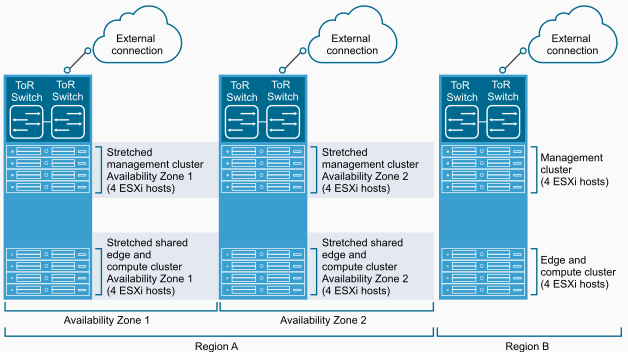
\includegraphics[width=0.95\textwidth]{imaxes/conceptosPrevios/zonasDispRegiones.png}
  \caption{Una región contiene al menos una zona de disponibilidad.}
  \label{fig:AVRegiones}
\end{figure}
\fi
%%%%%%%%%%%%%%%%%%%%%%%%%%%%%%%%%%%%%%%%%%%%%
%%%%%%%%%%%%%%%%%%%%%%%%%%%%%%%%%%%%%%%%%%%%%
%%%%%%%%%%%%%%%%%%%%%%%%%%%%%%%%%%%%%%%%%%%%%

\FloatBarrier

\subsubsection{Red física}
La topología de red en la capa física del SDDC de VMware Cloud Foundation se puede implementar mediante servicios de \underline{transporte} en la capa 2 o en la capa 3. El \underline{diseño en la capa 2} implica que la topología de la red incluya los dispositivos de capa 2 (\textit{Top of Rack Switches}) y los dispositivos de la capa 3 (routers, switches) [Fig. \ref{fig:transportlayer2}], por lo tanto las VLANs que se definan se deben implementar en la capa 2 y en la capa 3. Esto puede provocar problemas al aumentar el tamaño de la red ya que el número de VLANs disponible es más limitado, y problemas de compatibilidad ya que es posible que los dispositivos físicos tengan que ser del mismo proveedor. El \underline{diseño en la capa 3} implica que la topología de la red solo incluye a los dispositivos de capa 3 [Fig. \ref{fig:transportlayer3}]. Esto permite limitar la definición de VLANs a esa capa y el uso de enrutamiento dinámico con protocolos OSPF o BGP entre la capa 2 y 3. Así se consigue una mayor libertad a la hora de seleccionar los dispositivos físicos de red y que su configuración es más sencilla.
\begin{figure}[h!]
  \centering
  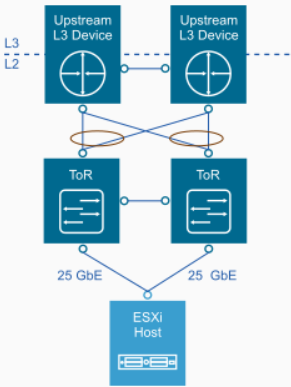
\includegraphics[width=0.3\textwidth]{imaxes/conceptosPrevios/transportlayer2.png}
  \caption{Límite de las capas 2 y 3 cuando la topología se implementa con dispositivos de capa 2.}
  \label{fig:transportlayer2}
\end{figure}
\FloatBarrier
\begin{figure}[h!]
  \centering
  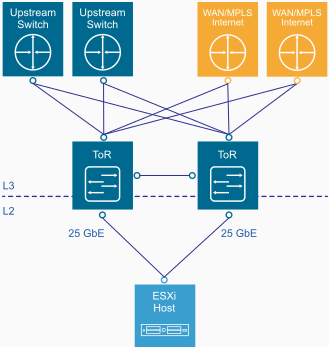
\includegraphics[width=0.3\textwidth]{imaxes/conceptosPrevios/transportNetLayer3.png}
  \caption{Límite de las capas 2 y 3 cuando la topología se implementa con dispositivos de capa 3.}
  \label{fig:transportlayer3}
\end{figure}
\FloatBarrier

\iffalse
n los componentes de VMware, o en la capa tres, para usar dispositivos de transporte lógico. Cada tipo de configuración tiene sus ventajas y desventajas, pero la configuración más común en este tipo de entornos es usar el transporte de red sobre la capa tres ya que da más libertad a la hora de gestionar y configurar los recursos físicos de red.\\
\fi

Como VMware Cloud Foundation abstrae la red física en una red virtual, la red física debe cumplir ciertos requisitos para que la red virtualizada sea robusta. Esta se debe mantener simple con configuraciones comunes en todos los switches, uso de VLANs y uso de enrutamiento dinámico, también debe ser escalable en cuanto a cantidad de hosts, ancho de banda y cantidad de rutas redundantes. Además, se debe tener en cuenta que cada tipo de tráfico tiene características diferentes, como por ejemplo el tráfico dedicado al almacenamiento a través de IP que suele usar mayor ancho de banda, por ello es necesario distinguir cada tipo de tráfico con protocolos \textit{Quality of Service} (QoS). El marcado de cada tipo de tráfico se realiza en el hipervisor ESXi a través de un vSphere Distributed Switch que soporta QoS tanto en la capa 2 como en la capa 3. En la capa 2 se utiliza  un campo de tres bits llamado \textit{Class of Service} que representa la prioridad del \textit{frame} con un valor de cero a siete, presente en la cabecera Ethernet cuando se utiliza etiquetado VLAN, mientras que en la capa 3 se utiliza un campo de 6 bits en la cabecera IP llamado \textit{Differentiated Services Code Point}, perteneciente al protocolo \textit{DiffServ}, para clasificar cada paquete. Los \underline{principales componentes que se deben configurar} para dar conectividad entre los servidores son los siguientes:
\begin{itemize}
    \item \textbf{Top of Rack Physical Switches} (TOR): es un switch al que se conectan los hosts de un rack para tener conectividad con el resto de la infraestructura. Se recomienda que un host esté conectado a dos switches TOR y que estos se configuren de forma redundante para proveer alta disponibilidad y tolerancia a fallos de alguna de las conexiones. Cada switch TOR se conecta a otro par de switches que establece conexión entre todos los racks.
    
    Los puertos del switch TOR que se conectan a los hosts deben estar configurados como puertos troncales de VLAN para que acepte todas las VLANs usadas por el host, se debe proveer servicio DHCP a cada VLAN usada y configurar los puertos para que acepten \textit{jumbo frames}. El marcado QoS del tráfico que realiza cada host ESXi debe ser aceptado y no puede ser modificado una vez abandona el host. \iffalse Además, se deben configurar todas las VLANs y subredes que se utilizarán en la infraestructura de VMware Cloud Foundation.\fi  
    
    \underline{Otros protocolos que se deben configurar} en los puertos que se conectan con los hosts son:
    \begin{itemize}
        \item \emph{Spanning Tree Protocol} (STP): protocolo que se encarga de gestionar las rutas de la red que son redundantes.
        \item \emph{Trunking}: configurar cada enlace troncal con las VLANs que van a transmitir tráfico a través de él. Se debe establecer como VLAN nativa, aquella utilizada para transmitir el tráfico que no tiene etiqueta, VLAN de la red \textit{management}.
        \item \emph{MTU}: configurar el MTU de cada VLAN para el transporte de paquetes \textit{jumbo frames}. Este valor será el que se use para configurar los hosts ESXi. Se recomienda establecerlo en 9000 bytes.
        \item \emph{Multicast}: configurar el protocolo IGMP en cada switch TOR como enrutador (busca activamente que VLANs pertenecen a un grupo Multicast) y cada VLAN como miembros de IGMP (los hosts que forman parte del grupo indican su pertenencia a un grupo multicast de forma activa).
    \end{itemize}
    

    
    \iffalse
    \item \textbf{Conectividad entre Regiones}: 
    \item \textbf{Conectividad entre Zonas de dispobilidad}:
    \fi
\end{itemize}

Los siguientes servicios usados por los componentes de VMware Cloud Foundation se deben configurar sobre la red física de la infraestructura para el correcto funcionamiento del SDDC\cite{CFexternalServices}:
\begin{itemize}
    \item \textbf{Servidor DNS}: se utiliza para obtener los nombres y direcciones de todas las máquinas virtuales que se creen, tanto en sentido \textit{fordward} (obtener una dirección IP a partir de un nombre) como en sentido \textit{reverse} (obtener un nombre a partir de una dirección IP). Además, este servicio debe ser configurado antes de realizar el despliegue de VMware Cloud Foundation. Este servicio es utilizado por el componente Platform Services Controller, vCenter Server, NSX Manager y vRealize Log Insight.
    
    \item \textbf{Servidor DHCP}: permite asignar direcciones IP de forma dinámica a los puertos \textit{vmkernel} de cada host ESXi. Este debe ser accesible desde cada VXLAN de VMware NSX y es necesario establecer previamente las redes que se van a usar en VMware Cloud Foundation. Este servicio debe estar disponible antes de comenzar el despliegue del SDDC ya que es necesaria la asignación dinámica de IPs.
    
    \item \textbf{Servidor NTP}: requerido por todos los componentes de VMware Cloud Foundation para mantener sus horas sincronizadas. Este servicio debe estar disponible en la infraestructura y configurado en cada host ESXi antes del despliegue de VMware Cloud Foundation, y debe ser alcanzable desde la red de \textit{management} y de vRealize. La derencia de tiempo entre los componentes de la infraestructura no debe ser mayor de cinco minutos.
    
    \item \textbf{Router}: debe existir enrutamiento dinámico en la red desde la capa 3. Es requerido por NSX para establecer comunicación con los ESG. Este servicio debe estar configurado antes del comenzar enl despliegue de VMware Cloud Foundation. 
\end{itemize}

\subsubsection{Host ESXi\cite{WDminRequierements}}
Los hosts ESXi que se desplieguen en un cluster deben tener características físicas idénticas para hacer la infraestructura más manejable,  incluyendo la configuración de almacenamiento y red. Para desplegar VMware Cloud Foundation se requiere:
\begin{itemize}
    \item  Dos interfaces de red (NIC) de la misma velocidad que deben estar conectadas a la VLAN troncal de dos switches TOR. Configurando \textit{NIC teaming} en VMware Sphere Distributed Switch se consigue que el tráfico se distribuya por las interfaces de red disponibles de forma óptima y que exista tolerancia a fallos.
    \item Todas las conexiones físicas del host deben tener al menos una velocidad igual a 10 Gbit.
    \item Cada host debe tener al menos 192 GB de memoria RAM, de esa cantidad, 176 GB de memoria RAM son requeridos por las máquinas virtuales que gestionan el SDDC.
    \item Un disco de arranque con un tamaño mínimo de 16 GB.
\end{itemize}

\subsubsection{Almacenamiento físico}
VMware Cloud Foundation utiliza VMware vSAN para proveer el almacenamiento de un SDDC. Para desplegar VMware Cloud Foundation, VMware vSAN requiere las siguientes características:
\begin{itemize}
    \item Mínimo de tres hosts con recursos de almacenamiento.
    \item Determinar qué configuración de vSAN se va a utilizar, \textit{All-Flash} o \textit{Hybrid}. Se recomienda la solución \textit{All-Flash} ya que ofrece mayor rendimiento.
    \item Para cada host con recursos de almacenamiento se debe cumplir que el disco de caché tenga un 10\% de la capacidad del almacenamiento persistente del grupo de discos, tener un mínimo de dos discos en la capa de capacidad, un controlador RAID y configurar habilitar vSphere High Availability  para apagar las máquinas virtuales de un host cuando este se encuentre aislado. El controlador RAID debe tener la característica \textit{pass-through} la cual permite que VMware vSAN muestre como discos individuales cada disco duro de un grupo de discos, esto facilita la gestión de cada disco y que se puedan realizar sustituciones sin detener el servicio.
    \item La capacidad mínima de almacenamiento disponible para el modelo consolidado es de 800 GB. 
\end{itemize}

\end{subsection}



%%%%%DISEÑO ARQ. VIRTUAL
\begin{subsection}{Arquitectura e Infraestructura Virtuales\cite{CFVirtInfraes}}
%%%%%%%%%%%%%%%%%%%%%%%%%%%%%%%%%%%%%%%%%%%%%
%%%%%%%%%%%%%%%%%%%%%%%%%%%%%%%%%%%%%%%%%%%%%
%%%%%%%%%%%%%%%%%%%%%%%%%%%%%%%%%%%%%%%%%%%%%
\iffalse
La infraestructura virtual de un SDDC puede estar formada por una o más regiones, cada una tiene su propio \textit{management domain} que contiene el \textit{management cluster}, y un \textit{virtual infrastructure domain} que contiene el \textit{shared cluster} y un \textit{compute cluster}.
\fi
%%%%%%%%%%%%%%%%%%%%%%%%%%%%%%%%%%%%%%%%%%%%%
%%%%%%%%%%%%%%%%%%%%%%%%%%%%%%%%%%%%%%%%%%%%%
%%%%%%%%%%%%%%%%%%%%%%%%%%%%%%%%%%%%%%%%%%%%%

Esta capa virtual provee infraestructura de almacenamiento, red y cómputo definida por software a través de servicios. En el modelo de despliegue consolidado de VMware Cloud Foundation, todos sus servicios y componentes se encuentran dentro de un mismo cluster (solo una AZ) dentro de la infraestructura, mientras que en el modelo estándar los servicios y componentes de gestión de la infraestructura están situados en clusters distintos (pueden estar en AZ distintintas), todos sus componentes se encuentran agrupados en un mismo cluster.



\subsubsection{Diseño de VMware vCenter Server}
El componente VMware vCenter Server es el punto de acceso y de control de todas las máquinas virtuales y servicios localizados en los hosts ESXi que forman parte de su dominio. En VMware Cloud Foundation se utiliza una instancia de VMware vCenter Server para controlar un \textit{workload domain} para aislar el flujo de trabajo y gestión de cada uno, simplifica la escalabilidad del SDDC, la gestión de actualizaciones para los componentes es más sencilla, permite determinar roles específicos y responsabilidades y permite aislar las redes de otras instancias de vCenter Server. Además, para gestionar vSpehere SSO Domain, VMware vCenter Server contiene embebido el componente PSC con todos los servicios necesarios.En caso de que existan varios \textit{Workload Domain} se puede habilitar el modo \textit{Enhanced Linked Mode} para poder gestionar todas las instancias de vCenter Server de forma centralizada desde un único vSphere Client.
Por lo anterior, en el \textit{management domain} se despliega una instancia de VMware vCenter Server que incluye un cluster de VMware vSphere.



%%%%%%%%%%%%%%%%%%%%%%%%%%%%%%%%%%%%%%%%%%%%%%%%%%%%%%%%%%%%%
%%%%%%%%%%%%%%%%%%%%%%%%%%%%%%%%%%%%%%%%%%%%%%%%%%%%%%%%%%%%%
%%%%%%%%%%%%%%%%%%%%%%%%%%%%%%%%%%%%%%%%%%%%%%%%%%%%%%%%%%%%%
%%%%%%%%%%%%%%%%%%%%%%%%%%%%%%%%%%%%%%%%%%%%%%%%%%
%%%%%%%%%%%%%%%%%%%%%%%%%%%%%%%%%%%%%%%%%%%%%%%%%%%%%%%%%%%%%
%%%%%%%%%%%%%%%%%%%%%%%%%%%%%%%%%%%%%%%%%%%%%%%%%%%%%%%%%%%%%

\subsubsection{Diseño cluster VMware vSphere}
Dentro de un \textit{workload domain} se pueden crear varios clusters vSphere con diferentes características. Para crear cluster y establecer sus características hay que tener en cuenta que se pueden usar menos hosts ESXi de mayor capacidad o más hosts EXi con menores prestaciones, el coste de cada host ESXi, el uso que se le va a dar al cluster y las características máximas y mínimas de un cluster vSphere. Para el \textit{management domain} se utiliza un único cluster vSphere con un mínimo de 4 hosts de los cuales se reserva un host para proveer redundancia. En caso de que el \textit{management domain} esté extendido en dos AZ entoces se requieren 4 hosts en cada AZ para proporcionar redundancia y disponibilidad en caso de caída de una de las AZ.
Dentro del cluster hay que configurar los servicios vSphere HA y vSphere DRS para proteger los componentes del SDDC. La configuración que se establece en el \textit{management domain} es la siguiente:
\begin{itemize}
    \item \textbf{vSphere High Availability}: en este servicio la propiedad \textit{Admission Control Policy} permite establecer la cantidad recursos reservados en caso de fallo y como se establece el cálculo de esos recursos. En el \textit{management domain} se configura para el fallo de al menos un host y reserva de recursos según un porcentaje, reservando así el 25\% de la CPU y el 30\% de la memoria RAM ya que funciona mejor cuando las VM usan mucha CPU y memoria. La otra propiedad que se debe habilitar para el correcto funcionamiento del servicio es \textit{VM and Application Monitoring}, que se encarga de reiniciar las VM en caso de caída.
    % que puede ser según el número hosts que pueden fallar en el cluster, según un porcentaje de reserva de rescursos o especificando el host donde se recolocan las VM del host caído.  RAM.  
    \item \textbf{vSphere DRS}: se activa usando la opción por defecto, \textit{Fully Automated} ya que aporta el mejor balance entre consumo de recursos y migraciones de VM innecesarias. Adicionalmente se pueden establecer reglas para determinar reglas de orden de encendido sobre grupos de VM. En caso de que exista más de una AZ, se deben crear grupos de VM y de hosts de cada AZ para luego implementar reglas de afinidad para que las VM de una AZ no sean migradas a otra AZ ya que esto puede afectar al rendimiento de la VM. 
\end{itemize}
% En el modelo consolidado se debe crear un único cluster con un mínimo de cuatro hosts ESXi ya que uno de los hosts se utiliza para asegurar la disponibilidad del almacenamiento vSAN cuando hay algún host inactivo. Este modelo proporciona capacidad de un único fallo por cluster.
\subsubsection{Diseño de red para el cluster vSphere}
Si bien en VMware Cloud Foundation existe VMware NSX-T, un componente dedicado únicamente a la administración de la red del SDDC, es desde VMware vSphere dónde se crean los elementos para formar las redes básicas que conectan los principales componentes del SDDC y para entregar y configurar sus servicios. Estas redes se configuran en base a los siguientes aspectos: 
\begin{itemize}
    \item Separar el tráfico de cada servicio para mejorar la eficiencia de la red y la seguridad. Así se puede ajustar las características de cada red, como el ancho de banda o la latencia, a las necesidades de cada servicio.
    \item Utilizar un único vSphere Distributed Switch por cluster donde se añade un \textit{port groups} por cada servicio.
    % \item Mejorar el rendimiento usando NICs de tipo VMXNET3 en las máquinas virtuales.
    \item Las NICs físicas de cada host ESXi conectados a un mismo vSphere Distributed Switch están conectadas también a la misma red física.
    % \item Aquellas redes que se dedican a servicios de la infraestructura deben estar configuradas con puertos tipo \textit{vmkernel}.
\end{itemize}
Para el \textit{management domain} del SDDC se crea un único vSphere Distributed Switch llamado \textit{sddc-vds01} con la siguiente configuración:
\begin{itemize}
    
    \item Se establece un MTU igual 9000 Bytes para permitir el tráfico de \textit{jumbo frames} ya que son requeridos por algunos de los servicios.
    
    \item Se habilita el servicio \textit{Network I/O} que permite establecer un nivel de prioridad a cada tipo de tráfico. Esto se realiza estableciendo limites de ancho de banda, políticas de balanceo de carga y reserva de recursos para un tipo de tráfico asociado a un servicio. Por cada tipo de tráfico hay cuatro aspectos que se pueden configurar que son \textit{Shares} (indica el \% de ancho de banda que se le da a un tipo de tráfico, el tipo de tráfico que tenga un mayor valor en \textit{Shares} tendrá más prioridad a la hora de usar los recursos), \textit{Reservation} (indica el valor de ancho de banda que se reserva para el tipo de tráfico) y \textit{Limit} (establece un valor máximo para el ancho de banda de un tipo de tráfico). En el \textit{management domain} los tipos de tráfico más relevantes que se deben configurar son los siguientes:
    \begin{itemize}
      \item \textit{Management Traffic}: el valor \textit{Shares} se establece al 50\% (\textit{Normal}) lo cual le da mayor prioridad que el resto de tipos. El resto de valores no se modifican.
      \item \textit{vSphere vMotion Traffic}: el valor \textit{Shares} se establece al 25\% (\textit{Low}) ya que durante el estado normal del entorno este tipo de tráfico no es muy importante. El resto de valores no se modifican.
      \item \textit{vSAN Traffic}: el valor \textit{Shares} se establece al 100\% (\textit{High}) para garantizar que este servicio recibe la cantidad de ancho de banda que necesita. El resto de valores no se modifican.
      \item \textit{Virtual Machine Traffic}: el valor \textit{Shares} se establece al 100\% (\textit{High}) para garantizar que las VMs siempre tienen acceso a la red ya que son una parte importante del SDDC. El resto de valores no se modifican.
    \end{itemize}
    
    \item Para detectar errores de compatibilidad entre la configuración del vSphere Distributed Switch y la red física se habilita el servicio \textit{Health Check}. Este se encarga de comprobar si la configuración de cada VLAN y MTU se adapta a la configuración de la capa física.
    
    \item Como puertos de salida \textit{Uplink} se configuran las dos interfaces físicas \textit{vmnic0} y \textit{vmnic1} de cada host.
    
\end{itemize}
En este vSpehere Distributed Switch para el \textit{management domain} se configuran los siguientes \textit{port groups}, que son del tipo \textit{Distributed port group} y del tipo \textit{Uplink port group}:
\begin{itemize}
       
        \item \textbf{Management port group}: es un \textit{Distributed port group} que comunica a todos los hosts ESXi entre si y transmite el tráfico entre los diferentes componentes de VMware Cloud Foundation, es decir, por este \textit{port group} circulan los comandos de configuración y gestión que los componentes del SDDC se envían entre ellos. Con el nombre \textit{sddc-vds01-mgmt}, en él están configurados los cuatro hosts ESXi y las VMs \textit{vcenter-mgmt}, \textit{sddc-manager}, \textit{nsx-mgmt-1},\textit{edge01-mgmt} y \textit{edge02-mgmt} bajo la subred con IP 10.0.0.0, con máscara de red 255.255.255.0, con VLAN 10 y con MTU igual a 1500 Bytes.
        
        \item \textbf{vMotion port group}: es un \textit{Distributed port group} que está dedicado al tráfico del componente vSphere vMotion para realizar las migraciones de máquinas virtuales de un host a otro. Con el nombre \textit{sddc-vds01-vmotion}, en él están configurados los 4 hosts bajo la subred con IP 10.0.4.0, con máscara de red 255.255.255.0, con VLAN 10 y con MTU igual a 8940 Bytes.
        
        \item \textbf{vSAN port group}: es un \textit{Distributed port group} que está dedicado al servicio de almacenamiento VMware vSAN y por él los hosts acceden al almacenamiento del SDDC. Con el nombre \textit{sddc-vds01-vsan}, en él están configurados los 4 hosts bajo la subred con IP 10.0.8.0, con máscara de red 255.255.255.0, con VLAN 10 y con MTU igual a 8940 Bytes.
        
        \item \textbf{Edge Uplink port group}: es un \textit{Distributed port group} dedicado a las conexiones del component NSX-T Edge que se dedica a dar acceso a determinados servicios y para proporcionar a otros \textit{workload domain} conexión con la red externa. Están gestionados por VMware NSX-T ya que dan servicio a sus componentes. En el entorno existen dos \textit{port groups} para proporcionar redundancia y alta dispobilidad, uno llamado \textit{sddc-edge-uplink01} cuyas instancias están configuradas bajo la red con IP 172.27.11.0 y con máscara de red 255.255.255.0, y otro llamado \textit{sddc-edge-uplink02} cuyas instancias están configuradas bajo la red con IP 172.27.12.0 y máscara de red 255.255.255.0. Ambos \textit{port groups} están configurados como VLAN Trunk (por ellos puede circular tráfico de cualquier VLAN) y tienen un MTU de 8940 Bytes. En los dos están configuradas dos VM llamadas \textit{edge01-mgmt} y \textit{edge02-mgmt}.
        
        \item \textbf{Uplink port group}: se trata de un \textit{Uplink port group} al que se le asignan las NICs físicas de cada host para establecer políticas sobre el tráfico que se dirige desde los hosts y VMs hacia fuera del vSphere Distributed Switch. Con el nombre \textit{sddc-vds01-DVUplinks-10}, en él están configuradas las dos NICs físicas de cada host, cada una en una interfaz \textit{uplink}.
        
\end{itemize}
La configuración que se aplica a cada \textit{Distributed port group} descrito anteriormente es la siguiente:
\begin{itemize}
  \item \textit{Port binding}: permite indidcar como se gestionan los puertos de un \textit{port group} cuando se añade o elimina una VM. Tiene dos opciones de configuración, la primera se denomina \textit{Static Port Binding} y su función consiste en asignar un puerto dentro del \textit{port group} a la VM que se conecta y solo se elimina cuando la VM es borrada. La segunda opción se denomina \textit{Ephemeral Port Binding} y consiste en que el puerto se asigna a la VM cuando esta se enciende y se elimina cuando se apaga o elimina. Para los \textit{port groups} \textit{sddc-vds01-vsan} y \textit{sddc-vds01-vmotion} se configura la opción \textit{Static Port Binding} ya que así se asegura que las VMs se conectan siempre al mismo puerto lo cual permite mantener datos históricos y hacer monitoreo a nivel de puerto. Para los \textit{port group} \textit{sddc-vds01-mgmt}, \textit{sddc-edge-uplink01} y \textit{sddc-edge-uplink02} se configura la opción \textit{Ephemeral Port Binding} ya que como el tráfico que circula por ellos es el que gestiona todos los componentes y da acceso a otras redes etonces se elimina la dependencia del estado de vCenter Server permitiendo que la comunicación continúe aunque vCenter Server no se encuentre operativo.

  \item \textit{Load Balancing}: indica como se distribuye el tráfico de salida de cada VM/host que se encuentran en el \textit{port group} entre las NICs físicas. Se selecciona \textit{Route based on physical NIC load}, es decir, el tráfico de una VM se transmite por una única NIC por lo que si esa NIC física está saturada, se asignará otra NIC física a la VM.
  
  \item \textit{Network failure detection}: esta opción permite establecer como debe determinar el \textit{port group} que alguna de las NICs físicas está fuera de servicio. Se selecciona \textit{Link status only} para que esto se determine según el estado que le transmite la NIC física, así se pueden detectar los fallos que ocurren en la red física.
  
  \item \textit{Notify switches}: si está habilitada, permite a los host enviar \textit{frames} a los switches físicos para que estos conozcan la localización de las VM que están funcionando en cada host. Se activa al seleccionar \textit{Yes}.
  
  \item \textit{Failback}: permite determinar como se reactiva una NIC cuando esta se recupera de un fallo. Al seleccionar \textit{Yes} se establece que la NIC se marcará como activa inmediatamente después de que se haya recuperado. Esta opción se debería desactivar en caso de que el estado de la NIC sea inestable.
  
  \item \textit{Failover Order}: permite determinar que uplinks se deben utilizar en cada estado de la conexión que puede ser \textit{active} (cuando los uplinks seleccionados están activos), \textit{stand by} (cuando alguno de los uplinks \textit{active} está incativo). Se seleccionan las dos interfaces \textit{uplink} disponibles en el estado \textit{active}. Para el \textit{port group} \textit{sddc-edge-uplink01} se selecciona la interfaz \textit{uplink1} como activa y se deja sin usar la interfaz \textit{uplink2}, mientras que se configura de forma contraria en el \textit{port group} \textit{sddc-edge-uplink02}.
\end{itemize}


%%%%%%%%%%%%%%%%%%%%%%%%%%%%%%%%%%%%%%%%%%%%
\subsubsection{Diseño de la red del SDDC con VMware NSX-T}
En un SDDC debe existir una red virtual, es decir, definida por software o también conocida como \textit{Software-Defined Network}. Esta red al estar construída con componentes de software, se desacopla de la red física sobre la que funciona lo que hace posible que se pueda modificar sin necesidad de cambiar la configuración en la capa física, reduciendo así la complejidad de la red física y el tiempo dedicado a la gestión de la misma. Además, este tipo de arquitectura habilita la posibilidad de implementar múltiples configuraciones de red en tiempo reducido proporcionando elasticidad y flexibilidad a la hora de administrar los recursos, tanto para el administrador como para el usuario final.
El componente encargado de crear, configurar y administrar la red virtualizada del SDDC es VMware NSX-T que a su vez contiene otros componentes entre los que se dividen distintas responsabilidades y funciones, ya descritos anteriormente.

%%%%% 1 - EXPLICACION DE LOS COMPONENTES DE NSX Y LOS QUE HAY EN EL ENTORNO
%%%%% 2 - COMO SE DEBE CONFIGURAR LA CAPA FÍSICA Y COMO ESTÁ IMPLEMENTADA EN EL ENTORNO ( parte de esto ya está definido en la parte de red física, REVISAR) => Meter la descripción de lo físico con el resto (modificar ese apartado) [https://docs.vmware.com/en/VMware-Validated-Design/6.0/sddc-architecture-and-design-for-the-management-domain/GUID-C924E896-D9C4-47BF-91D5-DF72605EF63E.html]
%%%%% 3 - REDES QUE HAY Y COMO SE EXTIENDEN ENTRE AZs
%%%%% 4 - COMO FUNCIONAN LAS COMUNICACIONES (GENEVE, ROUTING ...)

% En esta sección se describe como VMware Cloud Foundation abstrae la red física en un conjunto de recursos virtuales de red, utilizando los servicios de VMware NSX para crear una capa virtual independiente de la infraestructura física.
VMware NSX-T despliega en el \textit{management domain} despliega tres instancias de NSX-T Manager aunque en el entorno solo se despliega una llamada \textit{nsx-mgmt-1} para mejorar el rendimiento, y dos instancias de NSX-T Edge que en el entorno se denominan \textit{edge01-mgmt} y \textit{edge02-mgmt}, cada conjunto de instancias de cada componente forman un cluster donde cada VM está protegida por las funcionalidades vSphere HA y vSphere DRS para proveer alta disponibilidad del servicio y migrar las VMs a otra ubicación en caso de caída de una AZ o de un host. Estas VMs están conectadas al \textit{Distributed port group} llamado \textit{sddc-vds01-mgmt} que les permite comunicarse entre ellas y con vCenter Server, además las instancias de NSX-T Edge también están conectadas a otros dos \textit{Distributed port group} llamados \textit{sddc-edge-uplink01} y \textit{sddc-edge-uplink02}. Si existe más de una AZ, varios de los \textit{distributed port groups} se deben extender al resto de AZs para que en caso de que la primera AZ falle sus VMs se puedan migrar a otra AZ y sigan teniendo conectividad. Los \textit{port groups} que deberían estar extendidos en todas las AZ son el \textit{port group} \textit{sddc-vds01-mgmt} de cada AZ\footnote{Cada AZ tiene su propio \textit{Management port group}, entonces en cada AZ debe ser accesible el \textit{Management port group} del resto de AZs.}, los \textit{port group} \textit{sddc-edge-uplink01}, \textit{sddc-edge-uplink02} y \textit{port group} \textit{Edge Overlay}.

Los elementos que utiliza VMware NSX-T para crear una red independiente de la configuración de la red física son \textit{Segment} y \textit{Transport Zone}. Con estos componentes VMware NSX-T puede crear túneles que definen redes de capa 2 sin necesidad de realizar ningún cambio en la configuración de la red física.
\begin{itemize}
  \item \textbf{Transport Zone} (TZ): define el alcance de la red virtual. Pueden ser de dos tipos distintos, basada en VLAN o basada en Overlay. Una TZ se puede asignar a varios TN que tendrán acceso a los \textit{Segments} que funcionen en esa TZ. Un TN se conecta a una TZ a través de un N-VDS los cuales se pueden conectar a la vez a varias TZ de tipo VLAN pero solo a una TZ de tipo Overlay.
  
  \item \textbf{Segment}: también llamado \textit{Logical Switch}, representa un dominio de broadcast de capa 2 que forma parte de una \textit{Transport Zone}. El tipo de tráfico puede ser VLAN u Overlay dependiendo de como se haya configurado la \textit{Transport Zone} de la que forma parte. Las VMs de cada TN se pueden conectar a los \textit{Segments} situados en las \textit{Transport Zones} a las que el host está conectado. Estas VMs se pueden comunicar con el resto de VMs conectadas al mismo \textit{Segment}.
   
\end{itemize}

En el \textit{management domain} del entorno existen dos \textit{transport zones} diferentes:
\begin{itemize}
  \item \textit{mgmt-domain-m01-overlay-tz}:
    \begin{itemize}
      \item Tipo: Overlay
      \item Transport Nodes: \textit{edge01-mgmt}, \textit{edge02-mgmt}, \textit{esxi1}, \textit{esxi2}, \textit{esxi3} y \textit{esxi4}.
      \item Segments:
        \begin{itemize}
          \item \textit{mgmt-xRegion01-VXLAN}:
            \begin{itemize}
              \item VNI: 68589
              \item Subred: 10.60.0.0/24
              \item VMs: \textit{vrlcm} (10.60.0.60), \textit{vridm} (10.60.0.30)
              \item Descripción: se usa para desplegar las aplicaciones (algunos productos de VMware vRealize Suite lo utilizan) que deben ser accesibles desde todas las \textit{Regions} del SDDC, por lo tanto este \textit{segment} debe estar extendido en todo el entorno para que las VMs que se alojen en él puedan mantener la misma configuración de red independientemente del lugar físico donde se encuentren.
            \end{itemize}
          \item \textit{mgmt-Region01A-VXLAN}:
            \begin{itemize}
              \item VNI: 67588
              \item Subred: 10.50.0.0/24
              \item Descripción: su finalidad es alojar aplicaciones que sean accesibles desde una misma \textit{Region}. El alcance de estas aplicaciones está limitado a una \textit{Region} por lo tanto este \textit{segment} solo está extendido dentro de la misma.
            \end{itemize}
          \item \textit{sddc-host-overlay}:
            \begin{itemize}
              \item VNI: 67534
              \item Descripción: \textit{segment} usado por los componentes de VMware NSX-T para comunicarse entre los diferentes hosts ESXi.
            \end{itemize}
        \end{itemize}
    \end{itemize}
  \item \textit{sfo01-m01-edge-uplink-tz}:
    \begin{itemize}
      \item Tipo: VLAN
      \item Transport Nodes: \textit{edge01-mgmt} y \textit{edge02-mgmt}.
      \item Segments:
        \begin{itemize}
          
          \item \textit{VCF-edge-mgmt-cluster-segment-11}:
            \begin{itemize}
              \item VLAN: 11
              \item VMs: \textit{edge01-mgmt} (172.27.11.2/24) y \textit{edge02-mgmt} (172.27.11.3/24).
              \item Descripción: usado para transmitir el tráfico saliente hacia la red física.
            \end{itemize}
          \item \textit{VCF-edge-mgmt-cluster-segment-12}:
            \begin{itemize}
              \item VLAN: 12
              \item VMs: \textit{edge01-mgmt} (172.27.12.2/24) y \textit{edge02-mgmt} (172.27.12.3/24).
              \item Descripción: usado para transmitir el tráfico saliente hacia la red física.
            \end{itemize}
        \end{itemize}
      \end{itemize}
\end{itemize}

Las TZ, tanto las basadas en Overlay como las basadas en VLAN, sirven para comunicar TNs que se encuentran en distintas partes de la infraestructura física (por ejemplo, en distintos racks) como si estuvieran situadas en el mismo dominio broadcast de capa 2 físico. El primer tipo de TZ utiliza el protocolo Geneve para crear un túnel entre el origen y el destino, el cual encapsula en paquetes UDP el tráfico de L2 que generan las redes lógicas de VMware NSX-T añadiendo un identificador llamado VNI que indica a que \textit{segment} pertenece. Una TZ de tipo VLAN utiliza encapsula el tráfico saliente a la red física añadiendo un identificador de VLAN que es el mismo para todos los \textit{segments} que pertenecen a la misma TZ VLAN. 
Esta encapsulación tiene lugar cuando los paquetes salen de la interfaz de una VM y entran en el N-VDS del TN. Para ello, cada TN tiene dispositivo llamado \textit{Tunnel End Point} (TEP) al que se le asigna una dirección IP utilizada para enviar y recibir el tráfico entre VMs que se encuentran en el mismo \textit{segment} pero se alojan en TNs situados en redes L2 diferentes. Los TNs que son hosts ESXi obtienen su dirección TEP de un servidor DHCP\footnote{El servidor DHCP hace que se simplifique el proceso de configuración de un nuevo host ESXi ya que le asigna una dirección IP de forma automática.} mientras que los que son instancias de NSX-T Edge la dirección IP se asigna de forma manual. El TEP de cada TN tiene las siguientes direcciones IP:
\begin{itemize}
  \item \textit{esxi-1}: 172.16.254.10, 172.16.254.11 
  \item \textit{esxi-2}: 172.16.254.12, 172.16.254.13
  \item \textit{esxi-3}: 172.16.254.14, 172.16.254.15
  \item \textit{esxi-4}: 172.16.254.16, 172.16.254.17
  \item \textit{edge01-mgmt}: 172.27.13.2, 172.27.13.3
  \item \textit{edge02-mgmt}: 172.27.13.4, 172.27.13.5
\end{itemize}
En el entorno desplegado todos los TN se encuentran dentro de la misma red física. Esto implica que no se genere tráfico con los TEPs ya que todas las TZs funcionan sobre un único dominio broadcast.

Al crear un \textit{segment} dentro de una TZ, se configura un modo de replicación que indica como se retransmite el tráfico Broadcast, Multicast y Unknown Unicast propio del \textit{segment} cuando este tiene que viajar a un TN que está en una ubicación distinta en el medio físico.El modo de replicación que se utiliza en todos los \textit{segments} es \textit{Two-Tier Hierarchical Mode}. Este consiste en que cuando desde un TN se envía algún tipo de tráfico BUM de un \textit{segment} cuyos TNs están distribuídos en distintos puntos de la infraestructura física, el TEP del TN origen detecta que debe retransmitir el tráfico a una red externa, en la red externa se selecciona un TN que recibe el tráfico y lo reenvía al resto de TNs dentro del mismo dominio de red que deben recibir ese tráfico, así se reduce el número de paquetes que el TN origen debe enviar. El tráfico solo se enviará a los TN que contienen VMs que forman parte del \textit{segment} que lo genera. Es el componente NSX-T Controller quien se encarga de actualizar e indicar a los TNs toda la información para que esta comunicación sea correcta.

En cuanto al enrutamiento lógico, VMware NSX-T define routers virtuales que se encuentran embebidos dentro del hypervisor de cada host ESXi, igual que cada \textit{segment}. Esta característica permite definir \textit{gateways} para los \textit{segments} creados sin necesidad de modificar la configuración de la red física. En el \textit{management domain} se usa el modelo de enrutamiento de doble capa (\textit{Two Tier Routing}) que utiliza dos routers de dos tipos distintos lo que permite separar las tareas de administración de la infraestructura lógica de las de gestión de la infraestructura del usuario. Los routers desplegados son un \textit{Tier-0} llamado \textit{mgmt-domain-tier0-gateway} y otro router \textit{Tier-1} llamado \textit{mgmt-domain-tier1-gateway}. Cada router lógico está formado por los siguientes elementos:
\begin{itemize}
  
  \item \textbf{Distributed Router} (DR): que gestiona el enrutamiento y se a subredes a través de sus interfaces lógicas. Estas subredes pueden ser \textit{segments} u otro DR. A cada interfaz se le asigna una dirección MAC y una dirección IP que representa el \textit{gateway} de la subred. Este componente está distribuído en todos los TN, tanto hosts ESXi como instancias de NSX-T Edge manteniendo la misma configuración (interfaces,tablas de enrutamiento, etc.). Su función es redirigir el tráfico que recibe entre las interfaces que tiene disponibles, es decir, enruta el tráfico entre los diferentes \textit{segments} a los que está conectado el router \textit{Tier-0}.  
  
  \item \textbf{Service Router} (SR): proporciona servicios de red de forma centralizada (NAT, DHCP, Load Balancer, VPN, Gateway Firewall y Bridging L2) y proporciona acceso a la red externa. Este componente no está distribuído entre los diferentes TN, solo se se encuentra en las instancias de NSX-T Edge. Los servicios que proporciona solo se entregan a los recursos cuya red está gestionada por VMware NSX-T.
\end{itemize}

Las interfaces de cada router lógico son de los siguientes tipos:

\begin{itemize}
  \item \textit{External Interface}: se refiere a las interfaces que conectan con el dispositivo de la red física, normalmente un router.
  \item \textit{Internal Transit Link}: está interfaz conecta a todos los DR de \textit{Tier-0} distribuídos en cada TN con los SR formando una única red.
  \item \textit{RouterLink Interface}: interfaz que conecta un router lógico de \textit{Tier-1} con uno de \textit{Tier-0} a través de una subred generada por defecto (100.64.0.0/16).
\end{itemize}

Los routers lógicos creados para el \textit{management domain} en el entorno tienen la siguiente configuración:

\begin{itemize}
  \item \textbf{mgmt-domain-tier0-gateway}: su función consiste en proporcionar acceso a la red física.
    \begin{itemize}
      \item \textit{External Interfaces}\footnote{Estas direcciones corresponden a las interfaces de los TN NSX-T Edge que conectan con las interfaces Uplink sobre dos \textit{segments} de tipo VLAN.}: Dos que se conectan al \textit{segment} \textit{VCF-edge\_mgmt-edge-cluster-segment-11} (172.27.11.2 y 172.27.11.3) y dos que se conectan al \textit{segment} \textit{VCF-edge\_mgmt-edge-cluster-segment-12} (172.27.12.2 y 172.27.12.3).
      \item \textit{Internal Transit Link}: Usa la subred 169.254.0.0/24.
      \item \textit{RouterLink Interface}: Tiene la dirección 100.64.192.0/31.
      \item Configuración: se utiliza BGP para comunicarse con el router físico a través de las \textit{external interfaces} (en la configuración de BGP se establece 65003 como el \textit{autonomous system} local)\footnote{El uso de BGP simplifica la configuración de nuevas rutas cuando se añaden componentes al entorno, y que no se pierda la conectividad en caso de caída de alguna de las interfaces. El protocolo BGP también debe estar configurado en el router físico.}, se activa \textit{Inter SR iBGP} para establecer una comunicación mediante BGP entre las instancias distribuídas del componente SR de \textit{mgmt-domain-tier0-gateway}\footnote{Cada una se encuentra en una instancia de NSX-T Edge respectivamente.} para que se pueda seguir transmitiendo el tráfico en caso de que alguna de las interfaces de una instancia de NSX-T Edge esté fuera de servicio, se activa el protocolo ECMP para balancear el tráfico hacia la red física entre los caminos disponibles (existen cinco rutas posibles para alcanzar el router físico). 
      \item Configuración HA: determina el modo en el que se va a ejecutar el router de \textit{Tier-0}. En este caso se selecciona el modo \textit{active-active} el cual implica que las instancias de SR (una en cada nodo NSX-T Edge) funcionan ambas de forma activa, el tráfico que reciba cada una será encaminado por una subred diferente. Es por esto que el router lógico de \textit{Tier-0} no puede ofrecer servicios centralizados.
    \end{itemize}

  \item \textbf{mgmt-domain-tier1-gateway}: router de \textit{Tier-1} dedicado a gestionar el enrutamiento de las VMs de aplcaciones no dedicadas a la administración del SDDC. 
  \begin{itemize}
    \item \textit{Internal Transit Link}: Usa la subred 164.254.0.0/24.
    \item \textit{RouterLink Interface}: Tiene la dirección 100.64.192.1/31.
    \item \textit{Segment Interfaces}: conectado al \textit{segment} \textit{mgmt-Region01A-VXLAN} con la dirección IP 10.50.0.1, y al \textit{segment} \textit{mgmt-xRegion01-VXLAN} con la dirección IP 10.60.0.1.
    \item Configuración HA: determina el modo en el que se va a ejecutar el router de \textit{Tier-1}. En este caso se selecciona el modo \textit{active-stanby} el cual solo utiliza una de las dos instancias del SR de \textit{Tier-1} (cada una en un nodo de NSX-T Edge) por lo tanto el tráfico que reciba solo será encaminado por un único punto. Esto permite activar servicios centralizados, por lo tanto será \textit{mgmt-domain-tier1-gateway} y no \textit{mgmt-domain-tier0-gateway} el encargado de proporcionarlos.
  \end{itemize}
\end{itemize}

% Así como el componente DR de los routers de \textit{Tier-0} y de \textit{Tier-1} están distribuídos por todos los TNs (incluídas las instancias de NSX-T Edge), el componente SR solo se encuentra en las VMs de NSX-T Edge por lo tanto son estas VMs las que proporcionan los servicios centralizados de SR y acceso a la red externa del entorno. Además, para que los componentes lógicos tengan acceso a los \textit{segments} descritos, las instancias de NSX-T Edge están conectadas a dos TZs:
% \begin{itemize}
  
%   \item \textit{mgmt-domain-m01-overlay-tz}: esta TZ proporciona a las VMs del entorno a los servicios de los routers de \textit{Tier-0} y de \textit{Tier-1} y también permite que esos routers lógicos tengan acceso a los \textit{segments} donde se encuentran esas VMs. Se utiliza el tipo Overlay para que se puedan comunicar TNs que se encuentran en distintas redes físicas sin que la configuración de la red física sea compleja.
  
%   \item \textit{sfo01-m01-dge-uplink-tz}: esta TZ se utiliza para conectarse a la red física a través de un router físico. Se utiliza el tipo VLAN para encapsular el tráfico saliente hacia al router físico y porque las VLANs usadas en los \textit{segments} dentro de esta TZ se configuran también en la infraestructura física, por lo tanto no hace falta crear una capa física virtual con Overlay.
% \end{itemize}

Para gestionar las conexiones de cada TN, tanto para los nodos NSX-T Edge como para los hosts ESXi, VMware NSX-T introduce el componente llamado \textbf{NSX-T Virtual Distributed Switch} (N-VDS). Cada TN del entorno posee un N-VDS, este elemento conecta sus interfaces a los \textit{segments} que se configuran en cada TN y establece un mapeo con las interfaces \textit{uplink} que se utilizan para dirigir el tráfico de cada TZ hacia el exterior del TN. En el caso de las instancias de NSX-T Edge, los dos \textit{uplinks} están mapeados con las NICs físicas de cada host ESXi a través de los dos \textit{distributed port groups} de vSphere vDS (\textit{sddc-edge-uplink01} y \textit{sddc-edge-uplink02}) a los que están ancladas ambas VMs, es decir, un \textit{uplink} está mapeado con una NIC física del host ESXi. 
En las TZ de tipo VLAN, se utilizan plantillas \textit{Uplink Policy} para indicar como debe el N-VDS tratar el tráfico de la \textit{transport zone} a la que se asigna. En cada \textit{Uplink Policy} se especifican varias \textit{Teaming Policy}, el identificador VLAN que debe usar el N-VDS cuando tiene que enviar el tráfico fuera del TN y el MTU de los \textit{uplinks}. Una \textit{Teaming Policy} indica como el N-VDS utiliza los \textit{uplinks} para conseguir conexiones redundantes y balanceo de la carga, en una \textit{Uplink Policy} se especifica una \textit{Teaming Policy} por defecto y otras adicionales.
Para la TZ de tipo VLAN \textit{sfo01-m01-dge-uplink-tz} se especifica la siguiente \textit{Uplink Policy}:
\begin{itemize}
  \item Nombre: \textit{uplink-profile-13}
  \item Transport VLAN: 13
  \item MTU: 8940
  \item Teaming Policy: se especifican tres, una por defecto y dos adicionales:
    \begin{itemize}
      \item \textit{Default teaming}: \textit{Load Balance Source}, hace un mapeo uno a uno entre cada interfaz virtual de cada VM y uno de los \textit{uplinks} del N-VDS, así todo el tráfico correspondiente a esa interfaz se envía y recibe por el mismo \textit{uplink}.
      
      \item \textit{uplink1-named-teaming-policy}: \textit{Failover Order}, se establece un \textit{uplink}, \textit{uplink1} en este caso, como activo que se utiliza para enviar todo el tráfico, y una lista de \textit{uplinks} ordenados que se utilizan en caso de que el primero no esté disponible, vacía para esta \textit{Teaming policy}.
      \item \textit{uplink2-named-teaming-policy}: \textit{Failover Order}, donde el \textit{uplink} activo es \textit{uplink2} y la lista de \textit{uplinks} de reserva está vacía.
    \end{itemize}
\end{itemize}
A los \textit{segments} de esta TZ, \textit{VCF-edge-mgmt-cluster-segment-11} y \textit{VCF-edge-mgmt-cluster-segment-12} se les asignan las \textit{Teaming Policy} \textit{uplink1-named-teaming-policy} y \textit{uplink2-named-teaming-policy} respectivamente. Con esta configuración el tráfico de cada \textit{segment} circula por una única NIC física del host ESXi. Esto, junto con la configuración \textit{Failover Order} establecida para los \textit{port groups} \textit{sddc-edge-uplink01} y \textit{sddc-edge-uplink02} en el vSphere vDS,se consigue que el tráfico de salida hacia la red física perteneciente a los componentes de VMware NSX-T y todas las aplicaciones cuya red gestiona VMware NSX-T, sea distribuído por dos redes distintas proporcionando redundancia y disponibilidad del servicio en caso de que ocurra una caída de alguna de las conexiones.



Estas conexiones están gestionadas por un N-VDS dentro de cada instancia. Este switch lógico utiliza tres interfaces que se conectan a las diferentes redes lógicas. Para aquellas redes lógicas que requieren salida al medio físico ya sea para comunicarse con otros TN o para acceder a la red externa, el N-VDS utiliza finalmente el switch VDS de VMware vSphere que conecta con las interfaces físicas del host ESXi donde corre la instancia de NSX-T Edge.

la utilizan tres interfaces para  Estas interfaces son \textit{eth0} que se dedica a la red \textit{Management}, \textit{fp-eth0} y \textit{fp-eth1} que ambas se dedican a la conexión con cada uno de los \textit{segments} Uplink. 


*********************************************

%%%%%%%%
% Se recomienda que la red física siga una topología de tipo \textit{Leaf-Spine} donde existen swithces que se conectan a los hosts (\textit{leaf switches}), que a su vez se conectan a otra capa de switches (\textit{spine switches}) que finalmente conecta con la red principal del SDDC. Este tipo de topología permite medir mejor su rendimiento y facilita la escalabilidad de la infraestructura. En caso de existir varias AZ, debe existir una red física entre ellas cuya capa 3 funcione con enrutamiento dinámico para automatizar la resolución de problemas en caso de caída de alguna de las conexiones.
%%%%%%%%%

N

\iffalse
La información sobre VTEP existentes, la relación entre direcciones MAC de máquinas virtuales y dirección IP de VTEP, y relación entre direcciones MAC de máquinas virtuales y su IP, la poseen las instancias de NSX Controller en tres tablas: 
    \begin{itemize}
        \item \textit{VTEP Table}, relación entre un VTEP y la VXLAN que tiene acceso: VNI (ID del segmento), IP (dirección IP del VTEP), Segment (dirección IP del segmento), MAC (dirección MAC de la NIC física donde está configurado el VTEP).
        \item \textit{MAC Table}, relación entre la dirección MAC de una máquina virtual y el VTEP que le da acceso: VNI (ID del segmento), MAC (dirección MAC de la máquina virtual accesible por la VTEP-IP), VTEP-IP (dirección IP del VTEP que da acceso a la máquina virtual de la MAC indicada).
        \item \textit{ARP Table}, relación entre la dirección MAC y la dirección IP de una máquina virtual: VNI (ID del segmento), IP (dirección IP de la máquina virtual), MAC (dirección MAC de la máquina virtual).
    \end{itemize}
Estas tablas permiten reducir la cantidad de tráfico en la red ya que las máquinas virtuales y dispositivos de enrutamiento ya no requieren enviar tráfico Broadcast para obtenerla.
La comunicación directa entre máquinas virtuales situadas en distintos hosts ESXi se realiza con tráfico Unicast entre sus respectivos VTEP, pero una máquina virtual también puede enviar tráfico dirigido a todas las máquinas virtuales que pertenecen a su mismo Logical Switch, es decir, a las máquinas de la misma \textit{trasnport zone}, pero pueden situarse en segmentos de red físicos distintos. Este tipo de tráfico puede ser Multicast, Unknown Unicast y Broadcast (BUM), y en VMware NSX se puede gestionar con tres modos de replicación distintos\footnote{Al configurar un Logical Switch se elige uno de los modos.}, modo Multicast, modo Unicast y modo Híbrido.
    \begin{itemize}
        \item \textbf{Modo Multicast}: requiere que en la red física se haya configurado una IP multicast para cada VXLAN (es decir, Logical Switch), y el protocolo IGMP Snooping en los switches físicos para crear grupos multicast y que el tráfico sea más eficiente, esto habilita multicast entre los VTEP de la misma subred que el emisor. Para transmitir este tráfico a VTEPs situados en otros segmentos de red, se debe configurar el protocolo PIM para poder enrutarlo con los dispositivos de capa 3 físicos. Esta configuración no permite desacoplar la red lógica de la red física.\\
        Se puede establecer un grupo multicast por cada VXLAN, esto implica que un host solo recibirá tráfico si tiene al menos una máquina virtual en el grupo, pero requiere configurar muchos grupos. Otra opción es crear un grupo multicast para todas las VXLAN, se necesitan menos direcciones IP pero se genera más tráfico en la red.
    \begin{figure}[h!]
    \centering
    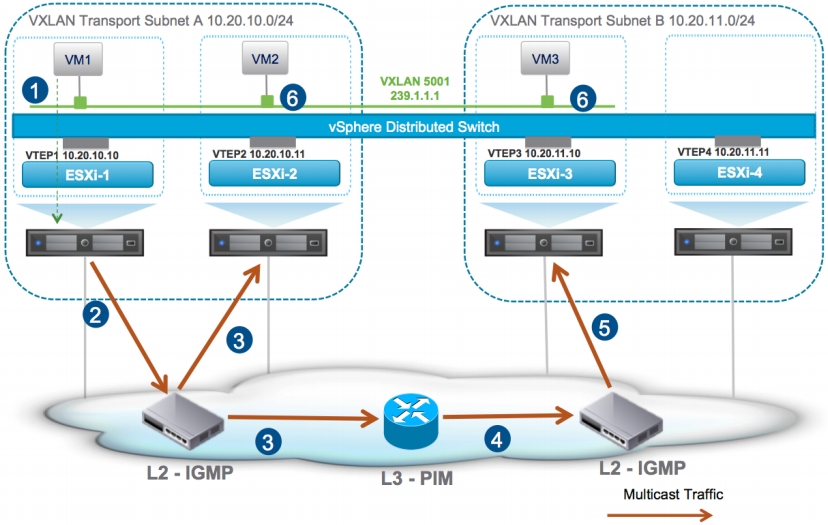
\includegraphics[width=0.5\textwidth]{imaxes/conceptosPrevios/MulticastSeqBUM.png}  \caption{Replicación del tráfico BUM en el modo Multicast}
    \label{fig:modoMulticast}
    \end{figure}
    \FloatBarrier
        \item \textbf{Modo Unicast}: no requiere ninguna configuración específica en la capa física y está gestionado por VMware NSX. Se crea un grupo con los VTEP situados en el mismo segmento de red, dentro de cada grupo se selecciona un host ESXi para el rol de \textit{Unicast Tunnel End Point} (UTEP), encargado de recibir el tráfico BUM que procede de otros segmentos de red para reenviarlo por su segmento pero solo a los hosts con al menos una máquina virtual. El host ESXi emisor utiliza la tabla VTEP para comprobar que VTEPs están situados en una VXLAN y así poder dirigir el tráfico BUM correspondiente.\\
        Este modo es útil en entornos pequeños donde no hay mucho tráfico y cada segmento de red tiene pocos VTEP.
    \begin{figure}[h!]
    \centering
    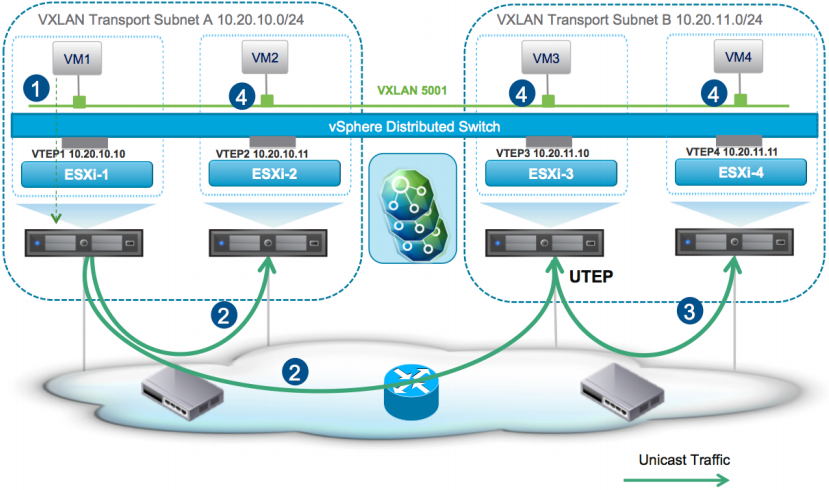
\includegraphics[width=0.5\textwidth]{imaxes/conceptosPrevios/UnicastMode.png}
    \caption{Replicación del tráfico BUM en el modo Unicast}
    \label{fig:modoUnicast}
    \end{figure}
    \FloatBarrier
        \item \textbf{Modo Híbrido}: combina el modo Unicast y el modo Multicast. El tráfico dirigido a las máquinas virtuales situadas en el mismo segmento de red se transmite usando Multicast, por lo que se requiere tener el protocolo IGMP configurado en los dispositivos físicos de capa 2, se recomienda establecer una dirección Multicast por cada VXLAN. El tráfico se replica a los hosts ESXi que forman parte del grupo. Cuando el tráfico va dirigido a máquinas virtuales situadas en hosts en distinto segmento de red, se transmite utilizando Unicast, como en ese modo, se forma un grupo con los hosts de cada segmento y de cada grupo se elige un host con el rol de \textit{Multicast Tunnel EndPoint} (MTEP). Así, el host que origina el tráfico BUM lo transmite al MTEP correspondiente, el cual se encarga de replicar ese tráfico por su segmento de red. La replicación del tráfico entre segmentos es gestionada por las instancias de NSX Controller.\\
        Este modo de replicación permite desplegar NSX en entornos grandes gracias a que el tráfico Multicast y Unicast se pueden escalar facilmente, el primero se reduce a cada segmento de red y la transmisión del segundo en la capa 3 está gestionado por VMware NSX sin necesidad de configurar los dispositivos físicos.
    \begin{figure}[h!]
        \centering
        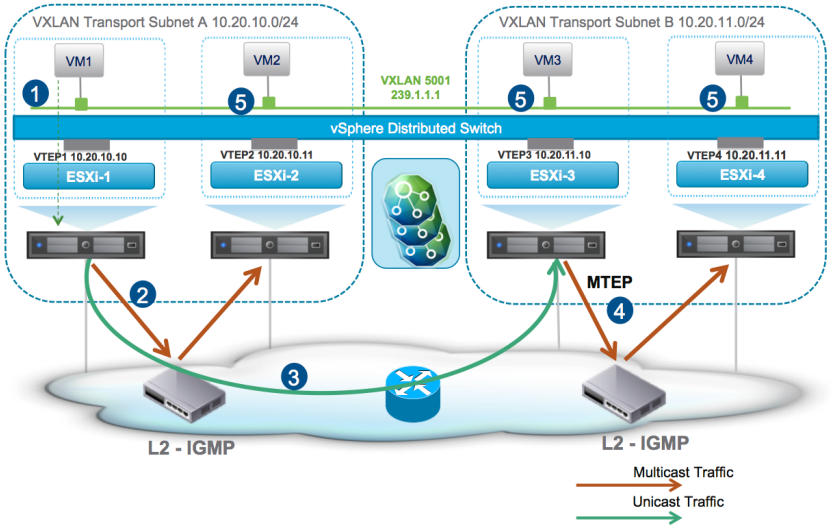
\includegraphics[width=0.5\textwidth]{imaxes/conceptosPrevios/hibrydMode.png}
        \caption{Replicación del tráfico BUM en el modo Híbrido}
        \label{fig:modoHibrido}
    \end{figure}
    \FloatBarrier
    \end{itemize}

 El enrutamiento del tráfico está gestionado por dos componentes Distributed Logical Router (DLR) y NSX Edge Services Gateway (ESG). Un mismo DLR se extiende por varios hosts ESXi para enrutar el tráfico entre VXLANs, también mantiene una conexión con las instancias de ESG para transmitir el tráfico que se dirige a redes externas, esa conexión se denomina \textit{transit network} y está getionada por un Logical Switch. Cada DLR tiene su propio Logical Router Control para intercambiar las rutas disponibles con las instancias de ESG, posteriormente, son las instancias de NSX Controller las que transmiten esta información al DLR distribuido en los hosts ESXi. Las interfaces lógicas del DLR conectan con cada Logical Switch, cada interfaz tiene una dirección IP que representa el \textit{gateway} del segmento de red al que esté conectada [Fig. \ref{fig:logicalRoutingCompo} y \ref{fig:redLogicaOne}]. Estos dispositivos utilizan enrutamiento dinámico (protocolos OSPF o BGP).
 
 \begin{figure}[h!]
  \centering
  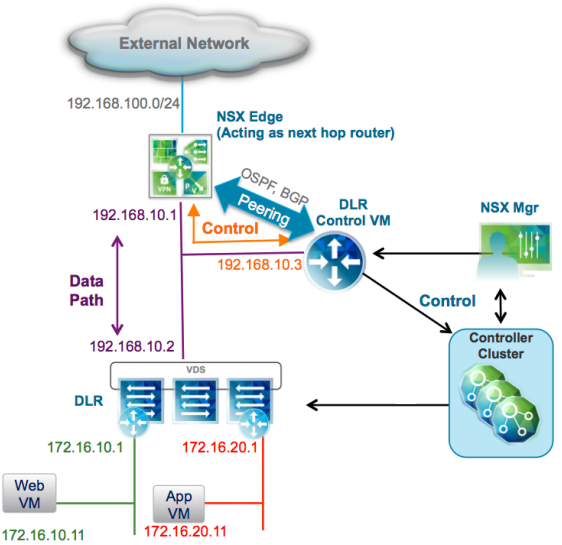
\includegraphics[width=0.4\textwidth]{imaxes/conceptosPrevios/LogicalRoutingComponents.png}
  \caption{Componentes de la red virtual que intervienen en el enrutamiento del tráfico.}
  \label{fig:logicalRoutingCompo}
\end{figure}
\FloatBarrier

\begin{figure}[h!]
  \centering
  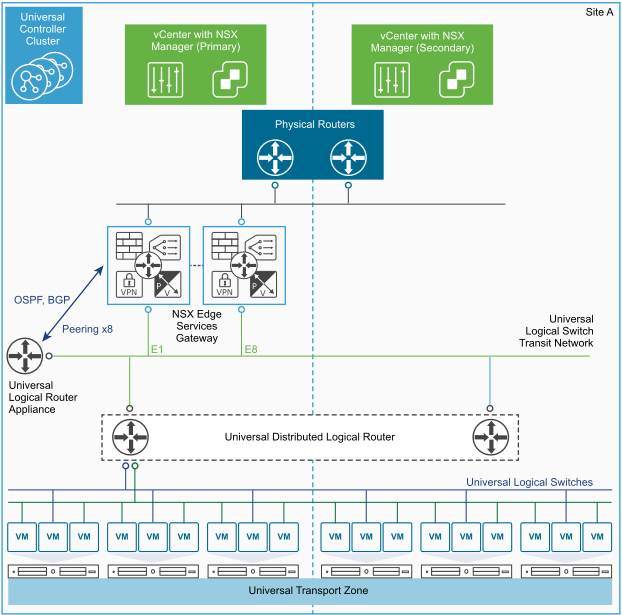
\includegraphics[width=0.5\textwidth]{imaxes/conceptosPrevios/redlogCF.png}
  \caption{Red lógica formada en un SDDC con dos clusters.}
  \label{fig:redLogicaOne}
\end{figure}
\FloatBarrier
 
 En el SDDC deben existir, al menos, dos intancias de ESG aunque se pueden desplegar hasta 8 instancias. En el modelo consolidado se debe tener un único UDLR para que las rutas entre hosts ESXi sean más cortas, debe existir un Logical Switch que forme la \textit{transit zone}. En el modelo estándar debe existir un UDLR extendido por todos los \textit{Management Cluster} (si hay varias \textit{Regions}), un UDLR extendido por el \textit{Shared Edge and Compute Cluster} y el resto de \textit{Compute Clusters} en cada \textit{Region}, y un DLR extendido por todos los clusters de una misma región.En el modelo estándar existen dos tipos de \textit{transit zones}, una entre el UDLR que atraviesa todas las \textit{Regions} y cada instancia de ESG, y otra que conecta el DLR propio de cada \textit{Region} y sus instancias de ESG. 
\\
Algunos componentes de VMware Cloud Foundation se deben desplegar en una VXLAN dedicada para proporcionar recuperación ante fallos en caso de que parte del SDDC deje de funcionar. Entre otros componentes (solo vamos a tratar aquellos que son obligatorios), VMware vRealize Log Insight se debe desplegar en una red de este tipo, llamada \textit{Application Virtual Network} (AVN). En entornos con varias \textit{Regions} se crea una \textit{transport zone} que se extiende por todo el SDDC y una \textit{transport zone} adicional en cada \textit{Region}, la primera proporciona recuperación ante fallos a través de todo el SDDC a los componentes que lo requieran, y la segunda solo a través de una \textit{Region}, sin necesidad de reconfigurar direcciones IP o DNS. VMware vRealize Log Insight se debe desplegar en una VXLAN por cada \textit{Region}.
\\
El acceso a una AVN se realiza a través de las instancias de ESG desplegadas en el entorno, estas se conectan a un UDLR que gestiona el tráfico de la s máquinas virtuales que tiene conectadas. El enrutamiento debe ser dinámico con BGP y las instancias de ESG proporcionan protegen y balacean la carga de trabajo con los servicios de VMware NSX Firewall y Load Balancing [Fig. \ref{fig:avnConsolidated}].\\
**VERIFICAR LO DEL LOAD BALANCING en el despliegue. ¿solo para las que son cross-region o tambien en las de una sola region**\\
\begin{figure}[h!]
  \centering
  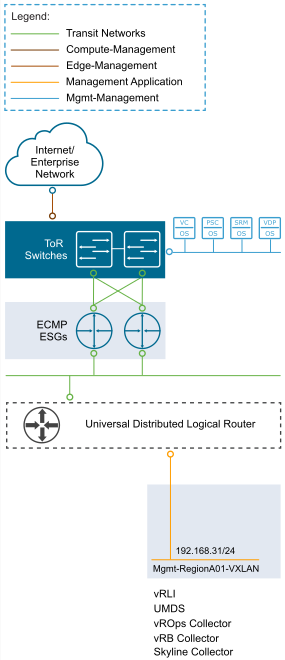
\includegraphics[width=0.25\textwidth]{imaxes/conceptosPrevios/AVNConsolidated.png}
  \caption{AVN en el modelo consolidado}
  \label{fig:avnConsolidated}
\end{figure}
\FloatBarrier

Este utiliza los componentes vCenter Server, NSX Manager, NSX Controllers y NSX Logical Switch para establecer comunicaciones y aislar los distintos tipos de tráfico [Fig. \ref{fig:planosNSX}]. Estos componentes \underline{actúan en diferentes planos} de la red:



\begin{itemize}
    \item \textbf{Plano de Datos}: esta capa gestiona la transmisión del tráfico entre los componentes del SDDC. En este plano actúan NSX Logical Switches segregando los tipos de datos, y el enrutamiento y firewall distribuído de NSX. Se transmite a través de una red física dedicada al transporte.
    \item \textbf{Plano de Control}: aquí se gestionan los mensajes de control que se usan para la configuración de los dispositivos de NSX como switches, routers y firewalls en cada host ESXi. Se distribuye en redes físicas de forma segura usando VLANs para aislarlo del plano de datos.
    \item \textbf{Plano de gestión}: aquí se gestiona el tráfico dedicado a la administración de los recursos como puede ser la creación y eliminación de máquinas virtuales. Está controlado por vCenter Server y NSX Manager.
\end{itemize}
\begin{figure}[h!]
  \centering
  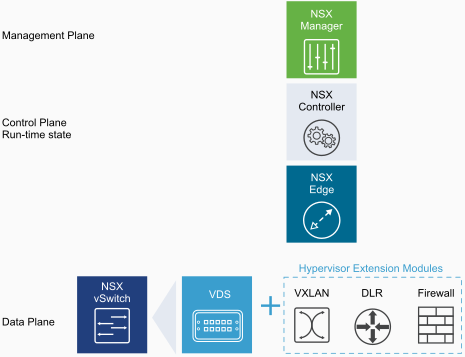
\includegraphics[width=0.65\textwidth]{imaxes/conceptosPrevios/planosNSX.png}
  \caption{Como se estructuran las componentes de VMware NSX for vSphere}
  \label{fig:planosNSX}
\end{figure}
\FloatBarrier

\fi

\iffalse
\subsubsection{Almacenamiento Virtual}
VMware vSAN forma único \textit{datastore} con todos los dispositivos de almacenamiento que se encuentran en la infraestructura permitiendo establecer políticas y gestionar esos recursos de forma más simple. Para que funcione correctamente es necesario \underline{configurar una red para VMware vSAN} teniendo en cuenta los siguientes aspectos:
\begin{itemize}
    \item El uso de vSpehere Distributed Switches genera mejor rendimiento.
    \item Se recomienda el uso de paquetes tipo \textit{jumbo frames}.
    \item Asignar una VLAN al tráfico de cada cluster de VMware vSAN.
    \item Si se implementa en un SDDC con dos localizaciones, es necesario establecer un host \textit{witness}.
\end{itemize}
Al establecer el tamaño y capacidad de este cluster hay que tener en cuenta que cuantos más hosts ESXi se incluyan, mayor tolerancia a fallos se tendrá y mejor se podrán repartir los grupos de discos entre todos los hosts. Debe haber un balance entre el hardware y la capacidad requerida.


\fi
\end{subsection}


\begin{subsection}{Operaciones de la Arquitectura\cite{CFopermanagement}}
En este apartado se define como se gestionan en VMware Cloud Foundation las tareas de administración de todas las partes de la infraestructura. Estas tareas se agrupan en la gestión del ciclo de vida y la recopilación de información sobre el estado de cada componente existente.

\subsubsection{Gestión del Ciclo de Vida}
Elementos que se encargan de administrar el ciclo de vida de los componentes:
\begin{itemize}
    \item \textbf{vSphere Update Manager}: por cada instancia de VMware vCenter Server se despliega una instancia de vSphere Update Manager. Este componente utiliza el servicio \textit{Update Manager Download Service} (UMDS) para obtener las actualizaciones de la red externa al SDDC, el cual se despliega en una red AVN [Fig. \ref{fig:avnConsolidated}], permitiendo limitar el acceso a Internet de vSphere Update Manager y reduciendo el número de descargas ya que un UMDS se comparte entre varias instancias de VMware vCenter Server. Se crea una instancia de UMDS por cada \textit{region} existente [Fig. \ref{fig:UpdateManagerArc}].
    \begin{figure}[h!]
        \centering
        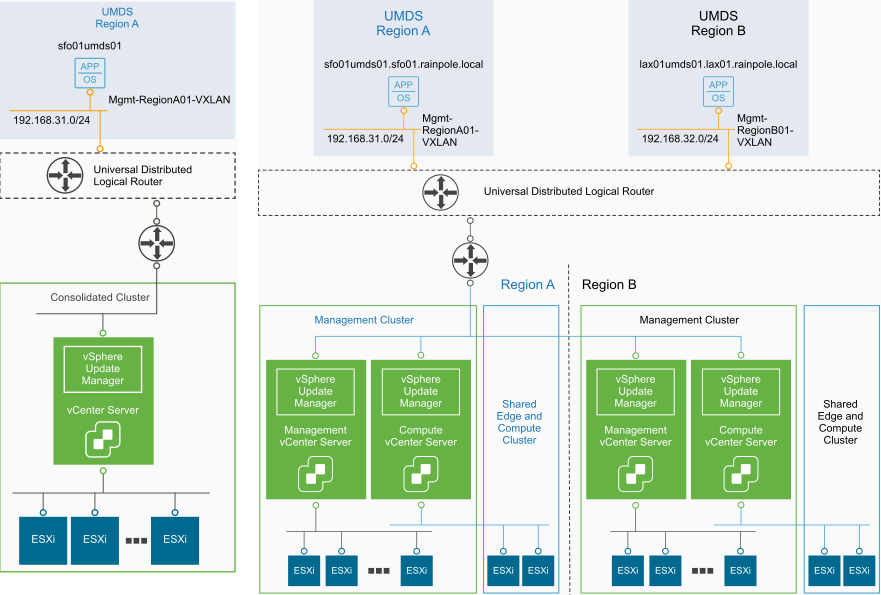
\includegraphics[width=0.5\textwidth]{imaxes/conceptosPrevios/UpdateManagerArch.png}
        \caption{Diseño de vSphere Update Manager en el modelo consolidado (izquierda) y en el modelo estándar (derecha)}
        \label{fig:UpdateManagerArc}
    \end{figure}
    \FloatBarrier
    
    \item \textbf{vRealize Suite Licfecycle Manager}: componente utilizado para desplegar, actualizar y configurar, de forma automatizada, los productos vRealize Operations, vRealize Log Insight, vRealize Automation y vRealize Business Cloud. De este componente se despliega una única instancia en una AVN accesible desde cada \textit{region} por todas las instancias de VMware vCenter Server. Se debe registrar su nombre de dominio en el servidor DNS para hacerla accesible.
    
    \iffalse
    y se puede elegir entre dos modelos de despliegue, uno en el que se usa una máquina virtual denominada  que se encarga de descargar los archivos requeridos por vSphere Update Manager mientras este se encuentra en un entorno aislado [Fig. \ref{fig:updateManager}], y otro donde es la instancia de vSphere Update Manager la que realiza la descarga de los ficheros. La primera opción incrementa la seguridad y permite compartir estos archivos entre distintas instancias de vSphere Update Manager.\\
    Una vez desplegado se pueden establecer diferentes configuraciones a nivel de host, máquina virtual y cluster, para que durante la instalación de actualizaciones el servicio del SDDC continúe operativo y evitar la pérdida de información y errores en los recursos.
    \begin{figure}[h!]
  \centering
  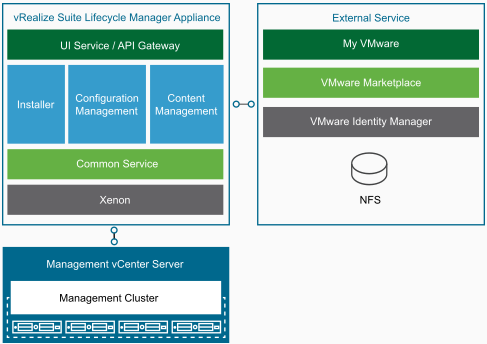
\includegraphics[width=0.8\textwidth]{imaxes/conceptosPrevios/vRealizeUpdateArchLifeCyle.png}
  \caption{Estructura de la gestión del ciclo de vida con vRealize Suite Lifecycle Manager.}
  \label{fig:vrealizeUpdateManager}
\end{figure}
\FloatBarrier
    \fi


\end{itemize}




\subsubsection{Gestión de Logs}
En VMware Cloud Foundation el producto vRealize Log Insight provee gestión y análisis de los logs de la infraestructura. Este componente resgistra los logs, alarmas y eventos de Platform Services Controller, instancias de VMware vCenter Server, de los hosts ESXi, componentes de VMware NSX, vRealize Suite Lifecycle Manager y componentes de vRealize Automation, utilizando el protocolo \textit{syslog} para su obtención. En el modelo consolidado se recomienda desplegar vRealize Log Insight en tamaño reducido, es decir, un solo nodo \textit{master} que gestiona los logs de todos los componentes, pero también se pueden desplegar otros nodos \textit{worker}. Para el modelo estándar se deben desplegar al menos tres nodos por cada \textit{region}, uno \textit{master} y dos \textit{worker}, y el uso de Load Balancer proporciona tolerancia a fallos en caso de que falle uno de los nodos. En ambos modelos los nodos se despliegan en una AVN que solo se extiende por una \textit{region} [Fig. \ref{fig:redLogIsight}], también se deben configurar la dirección IP y nombre de dominio de cada nodo en el servicio DNS.
    \begin{figure}[h!]
  \centering
  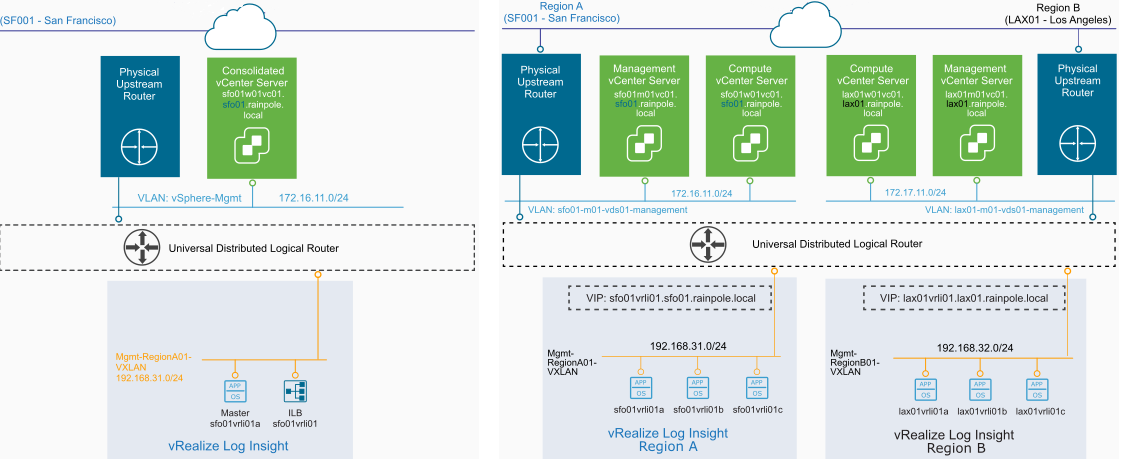
\includegraphics[width=0.7\textwidth]{imaxes/conceptosPrevios/networkLogInsight.png}
  \caption{Localización de vRealize Log Insight en el modelo consolidado (izquierda) y en el modelo estándar (derecha)}
  \label{fig:redLogIsight}
\end{figure}
\FloatBarrier
\end{subsection}
